\documentclass[a4paper,English,10pt]{article}
\usepackage[utf8]{inputenc}
\usepackage[T1]{fontenc}
%% \usepackage[English]{babel}     
\usepackage{graphicx,mathpple, textcomp, varioref}
\usepackage{fullpage}
\usepackage{fancyhdr}
\usepackage{lastpage}
\usepackage{hyperref}
\usepackage{amsmath}
\usepackage{braket}
\usepackage{enumitem}
\usepackage{booktabs}
\usepackage{subcaption}

\title{Fys4110: Project 2}
\author{Knut Halvor Helland}
\pagestyle{fancyplain}
\fancyhf{}
\renewcommand{\headrulewidth}{0pt}
\fancyfoot[R]{\thepage/\pageref{LastPage}}
\tolerance = 5000
\hbadness = \tolerance
\pretolerance = 2000
\setlength{\headheight}{20pt}

\newcommand{\unit}[1]{\; \mathrm{#1}}
\newcommand{\bb}[1]{\boldsymbol{#1}}
\newcommand{\p}{\partial}
\newcommand{\dd}{\mathrm{d}}
\newcommand{\ddt}[2]{\frac{\dd #1}{\dd #2}}
\newcommand{\dndt}[3]{\frac{\dd^{#3} #1}{\dd #2^{#3}}}
\newcommand{\pddt}[2]{\frac{\p #1}{\p #2}}
\newcommand{\pndt}[3]{\frac{\p^{#3} #1}{\p #2^{#3}}}
\newcommand{\Rar}{\Rightarrow}
\newcommand{\rar}{\rightarrow}
\newcommand{\uar}{\uparrow}
\newcommand{\lar}{\leftarrow}
\newcommand{\dar}{\downarrow}
\newcommand{\lagr}{\mathscr{L}}
\newcommand{\ham}{\mathcal{H}}
\newcommand{\id}{\bb{1}}
\newcommand{\deldt}[2]{\frac{\delta #1}{\delta #2}}
\newcommand{\be}{\begin{equation}}
\newcommand{\ee}{\end{equation}}
\newcommand{\f}{\frac}
\newcommand{\Det}{\mathrm{Det}}
\newcommand{\sgn}[1]{(-1)^{|#1|}}


\renewcommand{\bar}{\overline}
\renewcommand{\braket}{\Braket}

\begin{document}
\maketitle{}
\begin{abstract}
$\ldots$
\end{abstract}

\tableofcontents
\listoftables

\section{Introduction}
In this project I continue the study of many interacting particles in an isotropic two dimensional harmonic oscillator.
In project 1 \cite{proj1} I used Hartree-Fock methods to construct the Slater determinant of linear combinations of single
particle non-interacting states that minimized the energy. In this project I would like to improve this estimate of the ground state
by adding a Jastrow factor. Then the energy cannot be found with Hartree-Fock methods, but rather from direct integration of the Hamiltonean.
I will do this using the Metropolis algorithm to pick out integration points.
I will add a Jastrow factor with a free parameter, minimize the energy with respect to this parameter, and
then calculate the energy of this new approximation of the ground state.
In addition I will study the 2 particle case with a singly parametrized symmetric wavefunction instead of the Slater determinant.


\section{Physical Problem}
We will study several Coulomb-interacting electrons in an isotropic two dimensional harmonic oscillator.
The full Hamiltonean of the problem with $N$ particles and using atomic units is
\be
H = \sum_i^N -\f{1}{2}\nabla^2_i + \f{1}{2}\omega^2r^2_i + \sum_{i<j}^N\f{1}{r_{ij}}, \label{ham}
\ee
where $r_{ij} = |\bb{r}_i-\bb{r}_j|$.
The non-interacting hamiltonean
\be
H_0 = \sum_i^N -\f{1}{2}\nabla^2_i + \f{1}{2}\omega^2r^2_i,\label{ham0}
\ee
has as an analytical ground state solution (up to normalisation) the slater determinant
\be
\mathcal{A}\left(\psi_1\ldots\psi_N;\bb{r}_1\ldots\bb{r}_N\right) =
\left|\begin{matrix}
  \psi_1(\bb{r}_1)&\cdots&\psi_N(\bb{r}_1)\\
  \vdots&\ddots&\vdots\\
  \psi_1(\bb{r}_N)&\cdots&\psi_N(\bb{r}_N)\\
  \end{matrix}\right|,
\ee
where
\be
\psi_i(\bb{r}) = \chi_i\psi_{n_x,n_y}(\bb{r}) = \chi_iH_{n_x}(\sqrt{\omega}x)H_{n_y}(\sqrt{\omega}y)\exp(-\f{r^2}{2}),\label{spwf}
\ee
are the $N$ lowest energy single particle wave eigenstates.
The general ground state for the interacting case is not known.


\section{Trial wave functions}
\subsection{2 Particle Case}
For the two particle case I will aproximate the ground state with the parametrized trial wavefunction
\be
\psi_T = \exp\left(-\alpha\omega(r_1^2 + r_2^2) -\f{r_{12}}{1+\beta r_{12}}\right),\label{2pw}
\ee
with $\alpha$ and $\beta$ as free parameters.

\subsection{Slater case}

For the many particle case we will use the non-interacting ground state Slater determinant for a modified potential of strength $\alpha\omega$
multiplied with a Jastrow factor with one free parameter.
We could used Slater determinants from linear combinations of different non-interacting single particle states as found in \cite{proj1} by Hartree-Fock methods,
however this turned out to be too complicated too do in our timeframe. Instead we will compare the Hartree-Fock approach to adding a Jastrow factor to this modified ground state.

\be
\psi_T =  \mathcal{A}\left(\psi_1(\alpha)\ldots\psi_N(\alpha);\bb{r}_1\ldots\bb{r}_N\right)\prod_{i<j}^N\exp\left(-\f{a_{ij}r_{ij}}{1+\beta r_{ij}}\right),
\ee
where  $\psi_i$ is the non-interacting single particle state with the $i$th lowest energy,
and $a_{ij}$ is $1$ when the particles have anti-paralell spins and $1/3$ when paralell.
Since we are talking about spin $1/2$ electrons there are two spin configurations for each spatial configuration for the single particle states that go into the Slater determinant.
However the hamiltonean \ref{ham} is independent of spin. Wen can exploit this to simplify the wavefunction we use. If we let
the $N/2$ first particles be in one spin state and the next $N/2$ in the other we may use a product of Slater determinants with only the particles in the same spin state in each:
\be
\psi_T = \mathcal{A}\left(\psi_{1,\dar}(\alpha)\ldots\psi_{N/2,\dar}(\alpha);\bb{r}_1\ldots\bb{r}_{N/2}\right)\mathcal{A}\left(\psi_{1\uar}(\alpha)\ldots\psi_{N/2\uar}(\alpha);\bb{r}_{N/2+1}\ldots\bb{r}_N\right)\prod_{i<j}^N\exp\left(-\f{a_{ij}r_{ij}}{1+\beta r_{ij}}\right).\label{npw}
\ee
In the 2 particle case this reduces to equation \ref{2pw}.


\subsection{Steepest Descent}
To find the optimal values for $\alpha$ and $\beta$ start with an initial guess and traverse the parameter space by going down the steepest descent.
\be
\left(\begin{matrix}\alpha\\\beta\end{matrix}\right)_{n+1} =  \left(\begin{matrix}\alpha\\\beta\end{matrix}\right)_{n} - \gamma\nabla_{\alpha,\beta}\braket{E},
\ee
where $\gamma$ is a parameter of the search and $\nabla_{\alpha,\beta}$ is the gradient operator in parameter space.
From \cite{mortenbok} the derivatives are
\be
\pddt{\braket{E}}{\alpha} = 2\left(\braket{\f{1}{\psi_T}\pddt{\psi_T}{\alpha}E} - \braket{\f{1}{\psi_T}\pddt{\psi_T}{\alpha}}\braket{E}\right)
\ee
and 
\be
\pddt{\braket{E}}{\beta} = 2\left(\braket{\f{1}{\psi_T}\pddt{\psi_T}{\beta}E} - \braket{\f{1}{\psi_T}\pddt{\psi_T}{\beta} }\braket{E}\right)
\ee
The expressions in are case are found in appedices \ref{app2pab} and \ref{appnpab}.

\section{Monte-Carlo Integration}

% wavefunction, slater, jastrow
In this project I will estimate the energy of the trial wavefunctions with Monte-Carlo (MC) integration.
MC integration is a method of estimating the value of integrals on the form
\be
\braket{F} = \int F(x_1,\ldots,x_N)p(x_1,\ldots,x_N)\prod_{k=1}^N\dd x_k, \label{MCI}
\ee
where \(p(x_1,\ldots,x_N)\) is a probability density function.
MC integration is then based on drawing points $\bb{r}_i$ according to $p$ and evaluating $F$ in these points
\be
F_i \equiv F(\bb{r}_i).
\ee
Then defining
\be
\bar{F} \equiv \f{1}{N}\sum_{i=1}^N F_i
\ee
we have that
\be
\braket{F} = \lim_{N\rar\infty}\bar{F}.
\ee
Since we cannot draw infinite points we use $\bar{F}$ as an estimate of $\braket{F}$.

In order to estimate an integral in this way we thus need a method to draw positions according to $p$,
a way to compute $F_i$ and a way to estimate the error in the integration.





\subsection{The Metropolis Algorithm}

%% The Metropolis algorithm is an algorithm for computing expectation values for functions of many variables efficiently.
%% It is based on semi-randomly walking through the integration space and finding the value of the function at each point.
%% Let \(F(x_1,\ldots,x_N)\) be the function we wish to find the expectation value of. Then
%% \be
%% \braket{F} = \f{\int F(x_1,\ldots,x_N)p(x_1,\ldots,x_N)\prod_{k=1}^N\dd x_k}{\int p(x_1,\ldots,x_N)\prod_{k=1}^N\dd x_k}, \label{exp}
%% \ee
%% where \(p(x_1,\ldots,x_N)\) is the (generally) non-normalized probability density function. In our case \(p\) is \(|\psi|^2\).
%% One advantage with this method is that it does not require explicit normalization of the probalility density.
The Metropolis algorithm is a way to draw points according to a probability ensity function $p$. It is based on semi randomly-walking through
the space. One advantage of the method is that the pdf does not need to be normalised, which is convenient.
We can thus rewrite equation \ref{MCI} to
\be
\braket{F} = \f{\int F(x_1,\ldots,x_N)p(x_1,\ldots,x_N)\prod_{k=1}^N\dd x_k}{\int p(x_1,\ldots,x_N)\prod_{k=1}^N\dd x_k}. \label{exp}
\ee
One disadvantage is that
as the each point is only a relatively small step from the last the correlations between points are high enough that we have to take them into account.


\subsubsection{Detailed Balance}
The Metropolis algorithm may be derived by demanding that the Markov chain exhibits detailed balance.
The criterion for detailed balance is
\be
P(a)P(b|a) = P(b)P(a|b),
\ee
or rewritten
\be
\f{P(a)}{P(b)} = \f{P(a|b)}{P(b|a)}.
\ee
We may split \(P(a|b) = G(a|b)A(a|b)\), where \(G(a|b)\) is the probability of proposing a move from $b$ to $a$, while
$A(a|b)$ is the probability of accepting a proposed move from $b$ to $a$. The the detailed balance requirement may be rewritten as
\be
\f{A(a|b)}{A(b|a)} = \f{P(a)G(b|a)}{P(b)G(a|b)}.
\ee
Now we choose an acceptance ratio that satisfies this requirement. The Metropolis choice is to use
\be
A(a|b) = \mathrm{min}\left(1,\f{P(a)G(b|a)}{P(b)G(a|b)}\right).\label{arat}
\ee

So the Metropolis algorithm for drawing points from a probability distrobution is
\begin{enumerate}
\item
  Draw a proposed move from the proposal distribution.
\item
  Evaluate the acceptance ratio $a$ from equation \ref{arat}.
\item
  Draw a random number $0 \leq r < 1$ from a uniform distribution.
\item
  If $a>r$ accept the move. Else reject the move.
\item
  Save position
\item
  return to point 1.
\end{enumerate}
  
  

\subsubsection{Symmetric Proposal Density}

If the proposal probality $G(a|b) = G(b|a)$ the proposal distribution is called symmetric and drops out of the acceptance ratio.
Thus there is less to calculate for each loop in the algortihm. However symmetric proposal densities lead to many proposed steps being rejected,
and thus to higher corelations between the points.


\subsubsection{Importance Sampling}

If we instead choose a non-symmetric proposal distribution we may choose one to maximise the acceptancerate.
If we choose a proposal distribution so that the probability of proposing a move into an area with a higher probability is higher than
the probability of proposing a move into an area with a lower probability, in other words
if $P(a)>P(b)$ then $G(a|b)>G(b|a)$, we will increase the acceptance rate. We need to make sure that the proposal distribution preserves ergodicity,
which means that the whole space may be reached from any point with enought steps. So the probability of proposing a move into an area with lower probability must be non-zero.
The obvious way to ensure proposals into higher probability is to use the gradient of $p$:
\be
\f{1}{p}\nabla p = \f{1}{|\psi_T|^2}\nabla|\psi|^2 = \f{2}{\psi_T}\nabla\psi \equiv 2F, \label{eq:qforce} 
\ee
where I have used that the wavefunction is real. If we only move one particle at a time in one direction at a time we only the derivative with respect to
that particle in that dimension. 
One choice that uses this and preserves ergodicity is
\be
\bb{x}_{i,n+1} = \bb{x}_{i,n} + \sigma \chi + \sigma^2F(x_{i,n}),\label{eq:prop}
\ee
where $\chi$ is a random variable from a gaussian distribution about $0$ with standard deviation $1$.
From \cite{mortenbok} the proposal distribution from this rule is
\be
G(x_{i,n+1}|x_{i,n}) = \exp\left(-\f{(x_{i,n+1} - x_{i,n} - \sigma^2F(x_{i,n}))^2}{2\sigma^2}\right).
\ee
\subsection{Local Energy}
In quantum mechanics the probability distribution is given by $|\psi|^2$ and the expectation value for an operator $O$ is given by
\be
\braket{O} = \f{\int\psi^*O\psi\prod_i\dd x_i}{\int|\psi|^2\prod_i\dd x_i},
\ee
This is not exactly on the form of equation \ref{exp}, but it can be rewritten in terms of local variables given by
\be
O_L = \f{1}{\psi}O\psi, \label{localdef}
\ee
so that the expectation value is
\be
\braket{O} =  \f{\int|\psi|^2O_L\prod_i\dd x_i}{\int|\psi|^2\prod_i\dd x_i}.
\ee
So the expectation value of the energy is given by
\be
\braket{E} =  \f{\int|\psi|^2E_L\prod_i\dd x_i}{\int|\psi|^2\prod_i\dd x_i},
\ee
with
\be
E_L = \f{1}{\psi}H\psi, \label{localEdef}.
\ee



\subsubsection{2 Particle Case}
We might compute the local energy by numerical differentiation, however we will see that that is inefficient compared to calculating the derivative analytically.
In the two particle case with hamiltonean given by equation \ref{ham} and trial wavefunction by equation \ref{2pw} the anaytical expression for the local energy is
\be
E_L(\bb{r_1},\bb{r_2}) = \left[\f{1}{2}(1- \alpha)\omega(r_1^2 + r_2^2) + 2\alpha\omega\right]  - \f{a}{(1+\beta r_{12})^2}\left[\f{a}{(1+\beta r_{12})^2}+  \f{1}{r_{12}} - \f{2\beta}{(1+\beta r_{12})} -\alpha\omega r_{12}\right] + \f{1}{r_{12}},
\ee
as shown in appendix \ref{applap}.

\subsubsection{Slater Case}
In the $N$ particle case with hamiltonean given by equation \ref{ham} and trial wavefunction by equation \ref{npw} the local energy is given by

\be
E_L = -\f{1}{2}\left(\f{\nabla^2|S_\dar|}{|S_\dar|} + \f{\nabla^2|S_\uar|}{|S_\uar|} + \f{\nabla^2J}{J} +  \left(\f{\nabla|S_\dar|}{|S_\dar|} + \f{\nabla|S_\uar|}{|S_\uar|}\right)\cdot
\f{\nabla J}{J}\right) + \f{1}{2}\omega^2\sum_ir_i^2 + \sum_{i<j}\f{1}{r_{ij}},
\ee
where the expressions for the laplacians are derived in appendix \ref{applapn} and are too big to include here.

\subsection{Error Estimation and Blocking}

Let $\Set{F_i}$ be a finite set of consecutive measurements of the quantity $F$ on a system in equilibrium, in other words the probability distribution for the measurements is
independent of time. For a true average of $\braket{F}$ the error of each measurement is given by
\be
e_i = F_i - \braket{F},
\ee
while the error in the mean of the measurements $\bar{F}$ is given by
\be
E = \bar{F} - \braket{F}.
\ee
The variance of $F$ is given by
\be
\sigma^2_F = \braket{(F-\braket{F})^2} = \braket{e^2},
\ee
while the variance of $\bar{F}$ is given by
\be
\sigma^2_{\bar{F}} = \braket{(\bar{F}-\braket{F})^2} = \braket{E^2},
\ee
noting that $E = (\sum_ie_i)/n$ we see that
\be
\sigma^2_{\bar{F}} = \braket{\left(\f{1}{n}\sum_ie_i\right)^2} = \f{1}{n^2}\sum_{i,j}\braket{e_ie_j}.\label{sigmam}
\ee

\subsubsection[Uncorrelated Data]{Uncorrelated Data \footnote{This section is based on the treatment in \cite{errors}}}
For uncorrelated data
\be
 \braket{e_i e_j} = 0,
\ee
when $i\neq j$
and so equation \ref{sigmam} says
\be
\sigma^2_{\bar{F}} = \f{1}{n}\braket{e^2} = \f{1}{n}\sigma_F^2.
\ee
These quantities depend on the true average $\braket{F}$ and are thus unknown, so we instead look at the following known quantity
\be
d_i = F_i - \bar{F} = e_i - E, \label{residualdef}
\ee
with mean square
\be
\bar{d^2} = \f{1}{n}\sum_n(e_i - E)^2 = \f{1}{n}\sum_i e_i^2 - E^2.
\ee
We note that the true average of this is
\be
\braket{\bar{d^2}} = \sigma_F^2 - \sigma_{\bar{F}}^2 = (n-1)\sigma_{\bar{F}}^2,
\ee
or
\be
\sigma_{\bar{F}}^2 = \f{\braket{\bar{d^2}}}{n-1}.
\ee
We still don't know $\braket{\bar{d^2}}$, but we can estimate it with $\bar{d^2}$. And so our estimate of $\braket{E}$ is
\be
\braket{E} = \sigma_{\bar{F}} \approx \sqrt{\f{\bar{d^2}}{n-1}}.\label{errorest}
\ee

If the measurements come with errors the errors propagate as
\be
\sigma^2_{\bar{F}} = \f{1}{n^2}\sum_i\sigma_{F_i}^2.\label{errprop}
\ee

\subsubsection[Correlations and Blocking]{Correlations and Blocking \footnote {This section is based on \cite{block} } }

%%  Then as above the average of $\Set{F_i}$ $\bar{F}$ is an estimate of the true average of $F$ $\braket{F}$. An estimate of the error in this aproximation
%% is given by the standard deviation of $\bar{F}$ $\sigma_{\bar{F}}$. The variance in $\bar{F}$ is given by
%% \be
%% \sigma_{\bar{F}}^2 = \Braket{\bar{F}^2} - \braket{\bar{F}}^2,
%% \ee
%% expanding this we find
%% \begin{align*}
%%   \sigma_{\bar{F}}^2 &= \braket{\left(\f{1}{N}\sum_{i=1}^NF_i\right)^2} - \braket{\f{1}{N}\sum_{i=1}^NF_i}^2\\
%%   &=\f{1}{N^2}\sum_{i=1}^N\sum_{j=1}^N\left(\braket{F_iF_j} - \braket{F_i}\braket{F_j}\right)\\
%%   &= \f{1}{N^2}\sum_{i=1}^N\sum_{j=1}^N\mathrm{cov}(F_i,F_j).
%% \end{align*}
When the data is correlated $\braket{e_ie_j}$ is not generally $0$ and so equation \ref{sigmam} reads
\be
\sigma_{\bar{F}}^2 = \f{1}{n}\braket{e^2} + \f{2}{n^2}\sum_{i,j\neq i}\braket{e_ie_j}
\ee
The time independence of the pdf means that $\braket{e_ie_j}$ should only depend on the relative distance between $i$ and $j$
$t \equiv |i-j|$ \cite{block}. So we can define $C(t) = \braket{e_ie_j}$ and write
\be
\sigma_{\bar{F}}^2 = \f{1}{n}\left[C(0) + 2\sum_{t = 0}^{n-1}\left(1-\f{t}{n}\right)C(t)\right]. 
\ee
For finite correlation time there exists some $t = t_{max}$ for which $C(t>t_{max}) = 0$. If
\be
\sigma_{\bar{F}}^2 = \f{1}{n}\left[C(0) + 2\sum_{t = 0}^{t_{max}}\left(1-\f{t}{n}\right)C(t)\right]. \label{errvar}
\ee
We know how to estimate $C(0)$ from above, but $C(t>0)$ is more complicated.
The blocking method allows us to build $C(t>0)$ into a new $C(0)$ which we can estimate in the regular way.


If we transform the data set $\Set{F_i}$ into another set $\Set{\tilde{F}_i}$, where
\be
\tilde{F}_i = \f{1}{B}\sum_{j=1}^{B}F_{(i-1)B+j},\label{block}
\ee
where $B$ is a whole number called the block size. Call $\tilde{F}_i$ a block.
Expanding $\tilde{C}(0)$ we see that
\begin{align*}
  \tilde{C}(0) &= \braket{\tilde{F}_i^2}-\braket{\tilde{F}_i}^2\\
  &= \f{1}{B^2}\sum_{a,b}^B\braket{\tilde{F}_{i+a}\tilde{F}_{i+b}}-\braket{\tilde{F}_{i+a}}\braket{\tilde{F}_{i+b}}\\
  &= \f{1}{B^2}\sum_{a,b}^BC(|a-b|)\\
  &= \f{1}{B}C(0) + \f{2}{B}\sum_{t=1}^{B-1}\left(1-\f{t}{B}\right)C(t),
\end{align*}
and so
\be
\f{\tilde{C}(0)}{N/B} = \f{1}{N}\left[C(0) +\sum_{t = 1}^{B-1}\left(1-\f{t}{B}\right)C(t)\right],\label{blockvar}
\ee
comparing with equation \ref{errvar} we see that blocking has incorporated part of the error from correlations into $\tilde{C}(0)$! So, for an appropriate block size an improved estimate of the error is
\be
\sigma_{\bar{F}}^2 \approx \f{\sigma_{\bar{\tilde{F}}}^2}{N/B -1}.\label{errest}
\ee
To find the approriate block size we may plot this estimate as a function of block size, and choose a value where this seems to flatten. 

\section{Implementation}
The code is found at \url{https://github.com/khhelland/Fys4411/tree/master/2/src}.

\subsection{Structure}
The code is set up as two classes one for the two particle case and a generalisation for 2,6 or 12 particles.
The 2 particle class i called vmc and the many particles class is called slatervmc. Both classes are initialized with a steplenght, frequency,
variational parameters and a seed for the random number generator. To run the integration both classes have a member function called run, which takes
the number of MC cycles and a blocksize. The classes have public booleans that can be set to determine whether or not to switch on the interaction,
jastrow factor, importance sampling and, in the 2 particle case, numerical differentiation. Both classes have member functions that write the energies to file,
and functions that perform a steepest descent parameter optimization. Due to problems with the automatic steepest descent getting stuck in local minima or becomming unstable
there is a manual steepest descent which uses a static steplength and simply prints updated parameters untill stopped. The idea is to use it by starting it with a relatively large
stepsize, see how it behaves, and then try again with a better initial guess and smaller stepsize.

Due to time constraints the code is somewhat messy, but hopefully it is readable anyway.
Due to the time constraints not alot of time has been put into optimization, and there are several obvious inefficiencies.

\subsection{Paralellization}

To run several integrations in paralell I used OpenMPI. The file paramain.cpp includes the MPI commands necesary to set up paralell processes and collect the results.


\section{Results}
\subsection{Cost of numerical differentiation}
I timed the program with $10^7$ MC cycles without the jastrow factor or interaction with both analytical and numerical differentiation in local energy.
The analytical aproach took on average 3.32 s while the numerical approach took on average 11.78 s. I conclude that the analytical approach is more efficient and move forward
using only the analytical expressions.

\subsection{Blocking}
Plots of the estimated error as a function of blocksize are found in figures \ref{figblock2pJ} through \ref{figblock12pIsJ}.
\begin{figure}
  \begin{center}
    \fbox{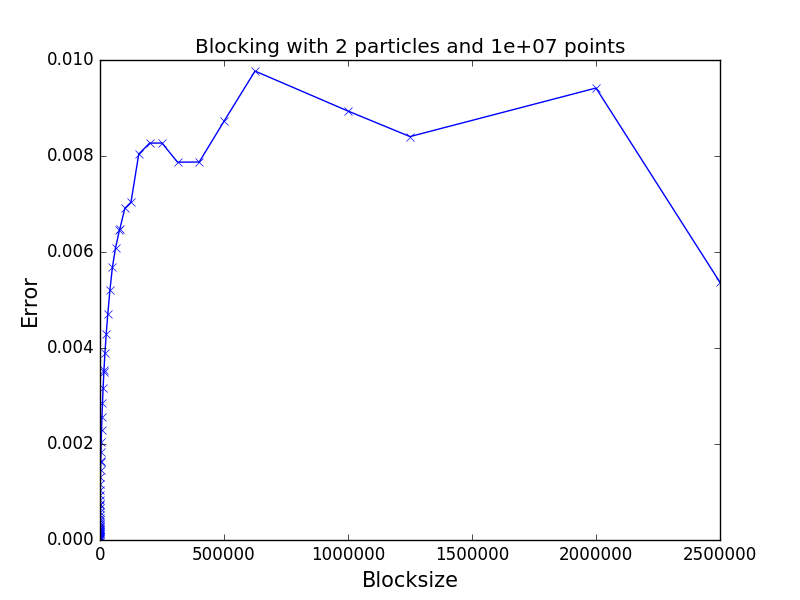
\includegraphics[width = 12cm]{block2pJ}}
  \end{center}
  \caption{Error as a function of block size for 2 particles with $1\times10^7$ MC cycles without importance sampling.
  The error seems to flatten after a blocksize of 250 000.}\label{figblock2pJ}
\end{figure}
\begin{figure}
  \begin{center}
    \fbox{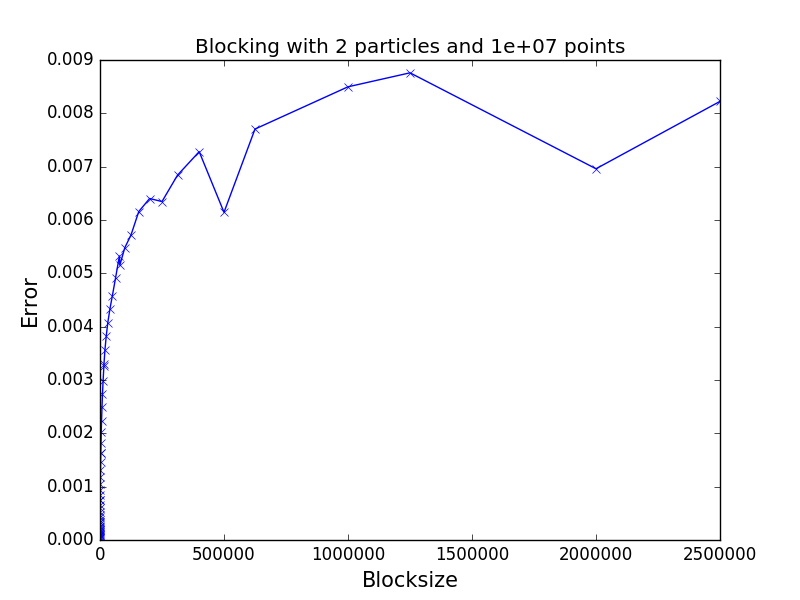
\includegraphics[width = 12cm]{block2pIsJ}}
  \end{center}
  \caption{Error as a function of block size for 2 particles with $1\times10^7$ MC cycles with importance sampling.
   The error seems to flatten after a blocksize of 200 000.}\label{figblock2pIsJ}
\end{figure}
\begin{figure}
  \begin{center}
    \fbox{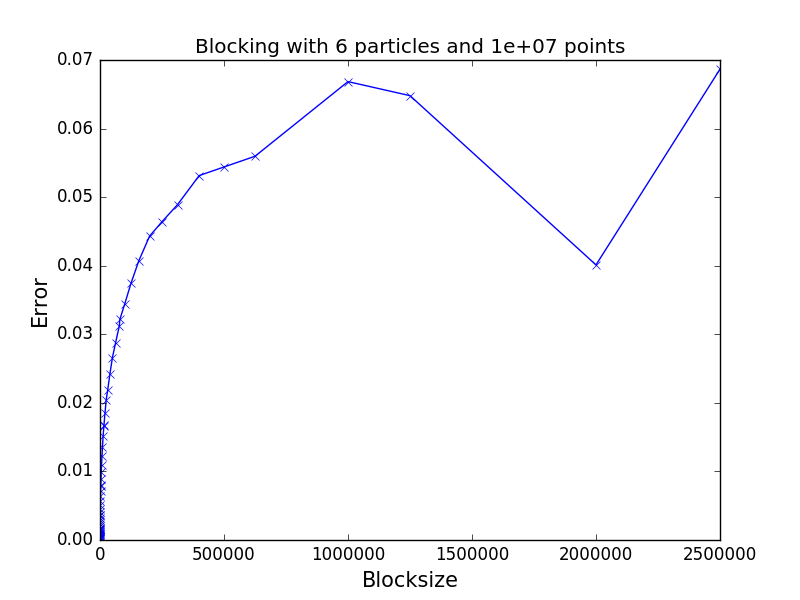
\includegraphics[width = 12cm]{block6pJ}}
  \end{center}
  \caption{Error as a function of block size for 6 particles with $1\times10^7$ MC cycles without importance sampling.
 The error seems to flatten after a blocksize of 400 000. }\label{figblock6pJ}
\end{figure}
\begin{figure}
  \begin{center}
    \fbox{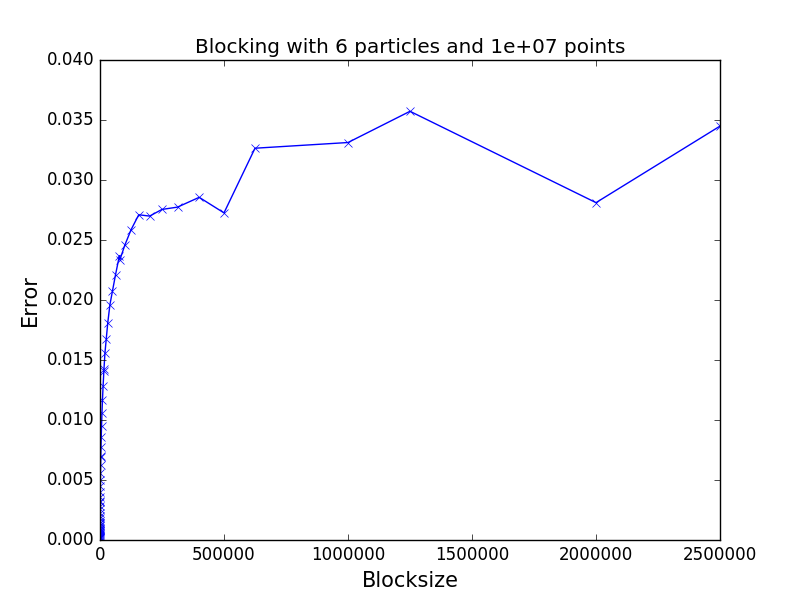
\includegraphics[width = 12cm]{block6pIsJ}}
  \end{center}
  \caption{Error as a function of block size for 6 particles with $1\times10^7$ MC cycles with importance sampling.
  The error seems to flatten after a blocksize of 156 250.}\label{figblock6pIsJ}
\end{figure}
\begin{figure}
  \begin{center}
    \fbox{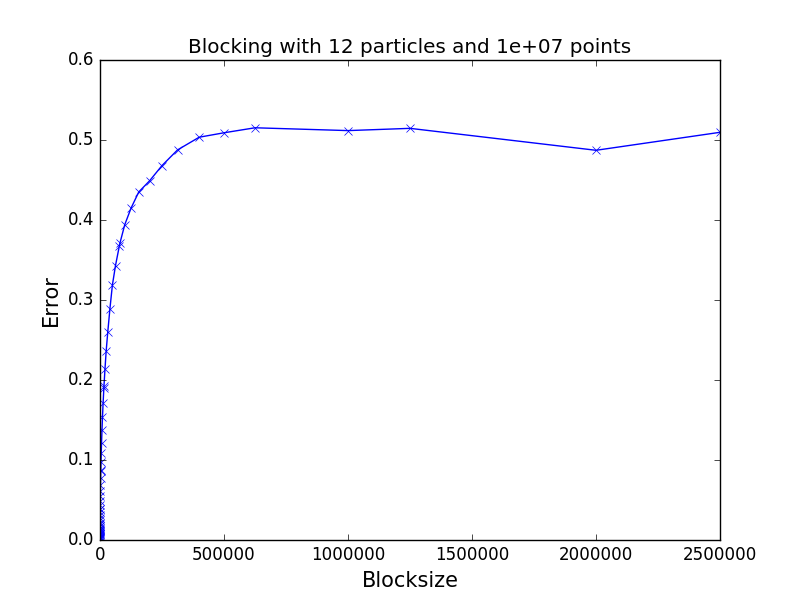
\includegraphics[width = 12cm]{block12pJ}}
  \end{center}
  \caption{Error as a function of block size for 12 particles with $1\times10^7$ MC cycles without importance sampling.
  The error seems to flatten after a blocksize of 500 000.}\label{figblock12pJ}
\end{figure}
\begin{figure}
  \begin{center}
    \fbox{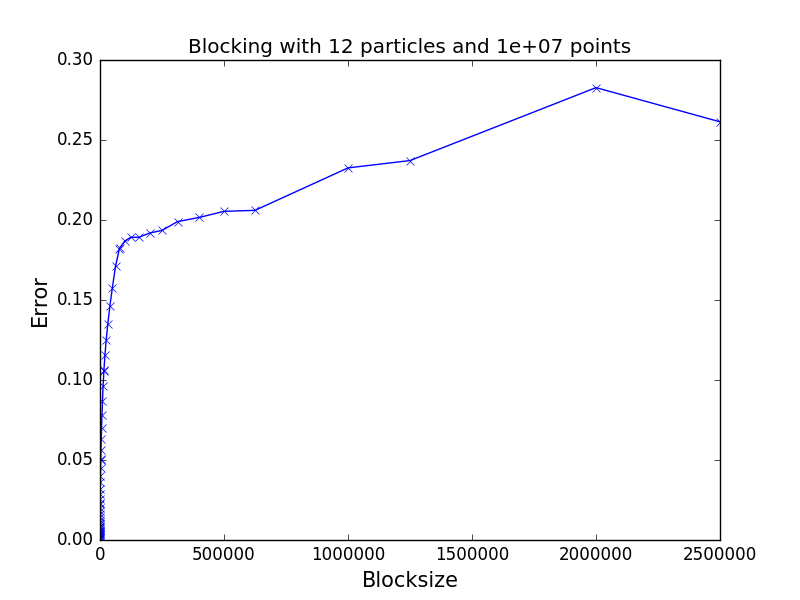
\includegraphics[width = 12cm]{block12pIsJ}}
  \end{center}
  \caption{Error as a function of block size for 12 particles with $1\times10^7$ MC cycles with importance sampling.
  The error seems to flatten after a blocksize of 100 000.}\label{figblock12pIsJ}
\end{figure}
In table \ref{blocktable} I have collected the blocksizes where the plots seem to flatten, and the blocksize I chose to work with.
I chose slightly bigger blocksizes than seem necessary from the plots.

\begin{table}
  \begin{center}
    \caption{Table of blocksizes. }
    \label{blocktable}
    \begin{tabular}{llcc}
      \toprule
      $N$ & importance samling? & blocksize from plot & chosen blocksize \\
      \midrule
      2 & no & 250 000 & 250 000\\
      & yes & 200 000 & 250 000\\
      \midrule
      6 & no & 400 000 & 500 000\\
      & yes & 156 250 & 250 000\\
      \midrule
      12 & no & 500 000 & 500 000\\
      & yes & 100 000 & 250 000\\
      \bottomrule
    \end{tabular}
  \end{center}
\end{table}



\subsection{Steepest Descent Optimization}
For the two particle case the automatic steepet descent algorithm seemed to work fine. It consistently found the same point
for a lot of different starting points, which seems to me to indicate that it really found a global minimum. However for the 6 and 12 particle
cases the automatic algorithm produced very eratic results, and I decided to do the search manually. This seemed to work for the case with no jastrow factor,
but failed with the jastrow factor. I discovered that the energy was very unstable as a function of the number of MC cycles, and that I probably needed
to use $10^7$ cycles to get reasonable results. One integral with $10^7$ cycles took about 1 minute for 6 particles and about 3 or 4 minutes for 12 particles.
Using this many points in a manual steepest descent search would be a grueling task, while an automatic search would have taken too much time. Therefore I decided
to just calculate the energy of a few parameter combinations chosen based on the optimal parameters for the two particle case and intuition and chose the set
that gave the lowest energy. Thus it may be a bit of a stretch to call these the optimal parameters. The parameters I ended up with are found in table \ref{paramtab}.



\begin{table}
  \begin{center}
    \caption{Table of ``optimal'' parameters found by steepest descent.}
    \label{paramtab}
    
    \begin{tabular}{*{5}c}
      \toprule
      $N$ & $\omega$ & $\alpha$ (no Jastrow) & $\alpha$ & $\beta$ \\
      \midrule
      2 & 1 & 0.767 & 0.985 & 0.402\\
      & 0.5 & 0.691 &  0.976 &  0.328\\
      & 0.1 & 0.511 & 0.948 & 0.170\\
      & 0.05 & 0.438 & 0.916 & 0.155\\
      & 0.01 & 0.278 & 0.940 & 0.097\\
      \midrule
      6 & 1 & 0.599 &  0.998 &  0.491\\
      & 0.5 & 0.532 & 0.956 & 0.475\\
      & 0.1 & 0.378 & 0.80 & 0.21\\
      & 0.05 & 0.314 & 0.5 & 0.15\\
      & 0.01 & 0.314 & 0.5 & 0.1\\
      \midrule
      12 & 1 & 0.556 & 1 & 0.4\\
      & 0.5 & 0.478 & 1 & 0.3\\
      & 0.1 & 0.313 & 0.8 & 0.2\\
      & 0.05 & 0.260 & 0.6 & 0.1\\
      & 0.01 & 0.150 & 0.1 & 0.1\\
      \bottomrule
    \end{tabular}
    \end{center}
\end{table}

\subsection{Benchmarks}
When the interaction is turned off, setting $\alpha = 1$ and turning off the jastrow factor make the trial wavefunctions \ref{2pw} and \ref{npw} the known ground states
with energies $2\omega, 10\omega$ and $28\omega$ for the 2,6 ans 12 particle case, respsectively. Since the ground state is an eigenstate the local energy for these states
should be equal to the total energy at every point. Thus the MC integration should find the exact energies with zero variance, yielding an error estimate of zero.
For these ground states it is also known that the expectation value for the kinetic and potential energies should be exactly half the total energy. However,
the states are not eigenstates for kinetic and potential energy, so we can not expect to find this exactly. We may use this to see how well the error estimation based
on blocking works, simply by comparing the deviation of the calculated values for $\bar{K}$ and $\bar{V}$ with the true means $\braket{K} = \braket{V} = \braket{E}/2$ and
the expected error. I have calculations with blocking and $10^7$ MC cycles for wavefunctions without jastrow factors, $\alpha = 1$ and no interaction in \ref{tabGround}. 
We see that in all cases $\bar{E} = \braket{E}$ exactly, with expected error equal to zero up to numerical precision. $\bar{K}$ and $\bar{V}$ are not exact, which is as expected,
but they deviate from their exact values by much more than the expected error, especially for low $\omega$.
\begin{table}
  \centering
  \caption[Results without jastrow factor or interaction]{Results from  calculations with blocking and $10^7$ MC cycles for wavefunctions without jastrow factors, $\alpha = 1$ and no interaction.}
  \label{tabGround}
  \begin{tabular}{*{9}c}
    \toprule
    N & $\omega$ & $\bar{K}$ & $\sigma_{\bar{K}}$& $\bar{V}$& $\sigma_{\bar{V}}$& $\bar{E}$  & $\sigma_{\bar{E}}$ &$\braket{E}$\\
    \midrule
    2 &1&1.05317	&0.00131343	&0.946828	&0.00131343	&2	&-1.13869e-16 &2\\
    &0.5&0.535774	&0.000661513	&0.464226	&0.000661513	&1&	0 & 1\\
    &0.1&0.106852	&9.89911e-05	&0.093148	&9.89911e-05	&0.2	&8.89602e-19 & 0.2\\
    &0.05&0.054874	&2.20498e-05	&0.045126	&2.20498e-05	&0.1	&8.89602e-20 & 0.1\\
    &0.01&0.0151137	&3.01902e-07	&0.00488625	&3.01902e-07	&0.02	&2.78001e-21  &0.02\\
    \midrule
    6&1&5.06396	&0.0234623	&4.93604	&0.0234623	&10	&3.64381e-16 &10\\
    &0.5&2.52148	&0.0100633	&2.47852	&0.0100633	&5	&-2.73286e-16 &5\\
    &0.1&0.570124	&0.000367148	&0.429876	&0.000367148	&1	&5.69345e-18  &1\\
    &0.05&0.333559	&6.76897e-05	&0.166441	&6.76897e-05	&0.5	&0      &0.5\\
    &0.01&0.0870228	&6.50881e-07	&0.0129772	&6.50881e-07	&0.1	&1.3344e-19 & 0.1\\
    \midrule
    12&1&13.8033	&0.121219	&14.1967	&0.121219	&28	&0 &28\\
    &0.5&7.01541	&0.0417814	&6.98459	&0.0417814	&14	&0 &14\\
    &0.1&1.51871	&0.00237558	&1.28129	&0.00237558	&2.8	&6.83214e-17 &2.8\\
    &0.05&0.835721	&0.000725358	&0.564279	&0.000725358	&1.4	&-3.98542e-17 &1.4\\
    &0.01&0.230431	&1.24871e-05	&0.0495693	&1.24871e-05	&0.28	&-3.55841e-19  &0.28\\
    \bottomrule
  \end{tabular}
\end{table}

When we turn on the interaction Taut has shown in \cite{taut} that the ground state energy for 2 particles and $\omega = 1$ is exactly 3 a.u..
Also \cite{mortenref} includes ground state energies for certain frequencies found by diffusion monte carlo methods. In \cite{proj1} I used Hartree-Fock methods to build a slater
determinant out of linear combinations of single particle wavefunctions and minimized the energy, which is another way to aproximate the ground state.
I have collected these results in \ref{tabMref}.

\begin{table}
  \centering
  \caption[Reference energies]{Reference values for ground state energies found by, diffusion monte carlo  collected from \cite{mortenref} (a), Hartree-Fock
    methods from \cite{proj1} (b) and the exact value for 2 particles and $\omega = 1$ from \cite{taut} (c).}
  \label{tabMref}
  \begin{tabular}{lllll}
    \toprule
    N&$\omega$&$\bar{E}_{a}$&$\bar{E}_b$&$E_c$\\
    \midrule
    2&1&3.00000 &3.16191 & 3\\
    &0.5&1.65975& 2.8386&\\
    6&1&20.1597&20.7192&\\
    &0.5&11.7888&17.8352&\\
    12&1&65.700&66.912&\\
    &0.5&39.159&56.6229&\\
    \bottomrule
  \end{tabular}
\end{table}

\subsection{MC Integration}
I ran the integration with $10^7$ MC cycles in 4 paralell processes. I assumed that the 4 results were uncorrelated when calculating the expected error, meaning I used equation
\label{errorprop}. I collected the results in tables \ref{Etab2},\ref{Etab6} and \ref{Etab12}.

\begin{table}
  \centering
  \caption[Results 2 particles]{Results of 4 paralell integrations with $10^7$ MC cycles each for 2 particles.
    The variation parameters chosen are those from table \ref{paramtab} and the expected errors have been calculated with the blocking method with blocksizes
    according to table \ref{blocktable}.The ``J?'' collumn indicates whether the jastrow factor was included or not.}
  \label{Etab2}
  \begin{tabular}{*{10}c}
    \toprule
    $\omega$ &J?& $\bar{K}$ & $\sigma_{\bar{K}}$& $\bar{V}$& $\sigma_{\bar{V}}$& $\bar{E}$  & $\sigma_{\bar{E}}$ & $\bar{r_{12}}$ &time\\
    \midrule
    1 &yes &0.896043	&0.0185009	&2.10496	&0.0183245	&3.001	&0.000765124	&1.64293&5.58495\\
    &no & 0.762656	& 0.0164748	& 2.37302	& 0.0257503	& 3.13568	& 0.0210561	& 1.44959 & 3.64587\\
    0.5 &yes& 0.442345	&0.0140292	&1.21753	&0.0136653	&1.65988	&0.00105956	&2.49304 &5.59341 \\
    &no & 0.339068	& 0.0106497	& 1.44792	& 0.0220222    &	1.78699 &	0.0200221 &	2.17777 & 3.76321\\
    0.1&yes &0.0854813	&0.00428608	&0.356026	&0.00398314	&0.441507	&0.000934913	&6.88561&5.64161 \\
    & no & 0.0449886& 0.00241899 &	0.465024 &	0.011365 &	0.510013 &	0.0110211 &	5.90909&3.67108\\
    0.05&yes &0.0373425	&0.00353373	&0.216955	&0.00317596	&0.254297	&0.000806016	&10.1328  &5.61539 \\
    &no&0.0192918	&0.00111495&	0.313173&	0.0112679&	0.332465	&0.0114061&	8.95725&3.63865\\
    0.01&yes &0.00715056	&0.000859333	&0.0695279	&0.000865545	&0.0766784	&0.000473462	&23.3606&5.547\\
    &no&0.00399493	&0.000103827	&0.125667	&0.00787434	&0.129662	&0.00790149	&15.8172&3.63274\\
    \bottomrule
  \end{tabular}
\end{table}

\begin{table}
  \centering
  \caption[Results 6 particles]{Results of 4 paralell integrations with $10^7$ MC cycles each for 6 particles.
    The variation parameters chosen are those from table \ref{paramtab} and the expected errors have been calculated with the blocking method with blocksizes
    according to table \ref{blocktable}.The ``J?'' collumn indicates whether the jastrow factor was included or not.} 
  \label{Etab6}
  \begin{tabular}{*{9}c}
    \toprule
    $\omega$ &J?& $\bar{K}$ & $\sigma_{\bar{K}}$& $\bar{V}$& $\sigma_{\bar{V}}$& $\bar{E}$  & $\sigma_{\bar{E}}$  &time\\
    \midrule
    1 &yes&3.68271	&0.06032	&16.5068	&0.0529771	&20.1895	&0.0145315&57.8832\\
    &no &2.99233	&0.0545036	&17.7254	&0.0956411	&20.7177	&0.0708336 &16.7907\\
    0.5 &yes&1.85946	&0.0391915	&9.998	&0.0339211	&11.8575	&0.0168981 & 60.13\\
    &no &1.32267	&0.0255294	&10.9755	&0.0623592	&12.2981	&0.0541781 &16.6152\\
    0.1&yes &0.296443	&0.0125718	&3.2867	&0.011232	&3.58314	&0.00453845 &57.2104\\
    & no & 0.206651	&0.00398447	&3.62807	&0.0352785	&3.83472	&0.0372295 &16.665\\
    0.05&yes &0.0682081	&0.0117284	&2.15215	&0.00884077	&2.22035	&0.0134219&62.8669\\
    &no&0.101616	&0.00179862	&2.48552	&0.0430841	&2.58714	&0.0442215 &17.0087\\
    0.01&yes &-0.138742	&0.0221044	&0.825324	&0.0161958	&0.686582	&0.00717069 &65.096\\
    &no&0.027521	&0.000172539	&1.68502	&0.0554644	&1.71254	&0.0555953  &16.6392\\
    
    \bottomrule
  \end{tabular}
\end{table}
\begin{table}
  \centering
    \caption[Results 12 particles]{Results of 4 paralell integrations with $10^7$ MC cycles each for 12 particles.
    The variation parameters chosen are those from table \ref{paramtab} and the expected errors have been calculated with the blocking method with blocksizes
    according to table \ref{blocktable}.The ``J?'' collumn indicates whether the jastrow factor was included or not.}
  \label{Etab12}
  \begin{tabular}{*{9}c}
    \toprule
     $\omega$ &J?& $\bar{K}$ & $\sigma_{\bar{K}}$& $\bar{V}$& $\sigma_{\bar{V}}$& $\bar{E}$  & $\sigma_{\bar{E}}$  &time\\
    \midrule
    1 &yes&8.54277&	0.13305	&57.6363	&0.124573&	66.179&	0.0544664 & 362.953\\
    &no &7.75721	&0.138949	&59.6794	&0.201069	&67.4366	&0.152718 &98.2915\\
    0.5 &yes&4.2585	&0.0757153	&35.2696	&0.0653093	&39.5281	&0.0356756 &357.436\\
    &no &3.21622	&0.0626376	&37.1745	&0.149676	&40.3907	&0.124732 &86.3928\\
    0.1&yes &0.600904	&0.0505859	&11.6492	&0.031241	&12.2501	&0.0245983 &360.226\\
    & no &0.541136	&0.010503	&13.0991	&0.14344	&13.6402	&0.1504 &86.9919 \\
    0.05&yes &-0.627686	&0.167751	&7.73977	&0.0363206	&7.11209	&0.159102  &407.275\\
    &no&0.276648	&0.00368362	&9.61352	&0.214207	&9.89016	&0.217163 &80.9301\\
    0.01&yes &-1.89996	&0.20771	&3.49049	&0.0992233	&1.59053	&0.111508 &389.397\\
    &no&0.0403921	&8.45161e-05	&7.47626	&0.28336	&7.51665	&0.283431 &84.4429\\
    \bottomrule
  \end{tabular}
\end{table}

\subsection{Onebody Densities}

The onebody density for a multiparticle wavefunction $\psi(\bb{r}_1,\ldots\bb{r}_N)$ is
\be
\int |\psi|^2\prod_{i = 2}^Nd\bb{r}_i\label{onebodyeq}.
\ee
Figure \ref{fig:onebody} shows the onebody density of the 2 particle trial wavefunction for $\omega = 1$ and optimal parameters both with and without the jastrow factor.
%% \begin{figure}
%%   \begin{center}
%%     \fbox{\includegraphics[width = 12cm]{}}
%%   \end{center}
%%   \caption{}\label{}
%% \end{figure}

\begin{figure}
  \centering
  \begin{subfigure}{0.5\textwidth}
    \centering
    \includegraphics[width=\linewidth]{2pdensity}
    \caption{With Jastrow}
    \label{fig:inclu}
  \end{subfigure}%
  \begin{subfigure}{0.5\textwidth}
    \centering
    \includegraphics[width=\linewidth]{2pdensityNoJ}
    \caption{Without Jastrow}
    \label{fig:deform}
  \end{subfigure}
  \caption{Onebody density for 2 particles, $\omega = 1$ with optimal parameters.}
  \label{fig:onebody}
\end{figure}
\subsection{Cost}

\subsection{Accuracy}


\section{Discussion}
\subsection{Errors}
As mentioned the kinetic and potential energy expectation values of harmonic oscillator eigenstates are exactly equal to half the energy.
Thus we know the absolute error of the estimates for kinetic and potential energy in table \ref{tabGround}. Comparing with the error estimates from the blocking analysis,
we see that the error estimates badly underestimate the true error. In fact they seem to miss by about an order of magnitude. The blocksize was chosen based on analysing calculations
of the total energy and so perhaps this only shows that I should have used a different blocksize based on what quantity I am looking at. But most of the correlations
should come from the points chosen from the probability distribution, the function we apply this too should not matter. Thus I think this may be an indication that I have
underestimated the errors even after blocking.

In tables \ref{Etab6} and \ref{Etab12} we see that for small $\omega$ and the Jastrow factor switched on $\bar{K}$ can be negative and the estimated error is too small to make up.
This is obviously wrong, and could indicate that there is a bug in the code and throw into question the rest of the results. However, I have already noted that the estimated error
for $K$ and $V$ is too small by at least an order of magnitude. Taking this into account makes $\bar{K} > 0$ be within the error. However it also means that the relative errors
for these calculations are so large that the values are effectively useless.

\subsection{Average distance between particles}
In the 2 particle case I included a calculation of the average relative distance of the particles, found in table \ref{Etab2}.
We see that the distance increases dramatically when $\omega$ decreases, and that the distance is greater in cases where the jastrow factor is included.
In figure \ref{fig:onebody} we saw that the onebody density was more condensed about the origin with the jastrow factor than without. These results seem
contradictory at first glance, but I suppose there are details in the wavefunction that are missed by simply looking at a plot of the onebody density.

\subsection{Comparison of results with and without Jastrow factor}
Looking at tables \ref{Etab2}, \ref{Etab6} and \ref{Etab12} we see that the energy estimates $\bar{E}$ are consistently lower when the jastrow factor is used.
The jastrow factor seems to be more important for higher numebers of particles and lower $\omega$. This makes sense as the factor is supposed to account for the interactions
of the particles, which naturally are more important the more particles there are and the stronger the interaction is compared to the confining potential.

\subsection{Comparison of results with benchmark values}
Comparing the results to table \ref{tabMref} we see that in the 2 particle case the energies with the jastrow factor are equal to the diffusion MC results within the errors.
For 6 and 12 particles the diffusion MC energies are mostly outside of the error ranges of my results. This is probably due to the parameter optimization not working as well
as I had hoped, but could also be a reflection of an overoptimistic estimation of the error. If we compare instead with the Hartree-Fock results we find that my results
give lower energies both with and without the jastrow factor, especially for $\omega = 0.5$.

\section{Conclusion}



\appendix
\section{A Note About Cofactors and Determinants}\label{cofac}
Determinants can be somewhat hard to work with, following \cite{mortenbok} we may use cofactors to do some trickery.
For a matrix $A$ with elements $A_{ij}$ the cofactors $C_{ij}$ are given by $(-1)^{i+j} M_{ij}$, with $M_{ij}$ being the determinant of the matrix formed by deliting the $i$th
row and $j$th collumn from $A$. There two properties of cofactors that will be important here are
\be
|A|\id = A C^T \Leftrightarrow |A| = \sum_jA_{ij}C_{ij},
\ee
and thus
\be
A^{-1} = \f{1}{|A|}C^T \Leftrightarrow A^{-1}_{ij} = \f{1}{|A|}C_{ji},
\ee
and the fact that $C_{ij}$ is independent of row $i$ and collumn $j$ of A.





\section{Derivatives of the 2 particle trial wavefunction}
In the course of the project we needed analytical expressions for different derivatives of the 2 particle trial wavefunction \ref{2pw}. I have collected
the differentiations here.

\subsection{Gradient}\label{app2pg}
In order to compute the driftforce for importance sampling we needed
\[\f{1}{\psi_T}\pddt{\psi_T}{z},\]
where \(z_i = x_1,x_2,y_1,y_2\).
As \(\psi_T\) is an exponential
\begin{align*}
  \f{1}{\psi_T}\pddt{\psi_T}{z_i} &= \pddt{}{z_i}\left(-\f{1}{2}\alpha\omega(r_1^2+r_2^2) + \f{ar_{12}}{1+\beta r_{12}}\right)\\
  &= -\alpha\omega z_i + a\left(\f{1}{1+\beta r_{12}} - \f{r_{12}\beta}{(1+\beta r_{12})^2}\right)\pddt{r_{12}}{z_i}\\
  &= -\alpha\omega z_i + \f{a}{(1+\beta r_{12})^2}\pddt{r_{12}}{z_i}\\
  &= -\alpha\omega z_i + \f{a}{(1+\beta r_{12})^2}\f{(z_i-z_j)}{r_{12}},\\
\end{align*}
where \(z_j\) is the coordinate of the other particle along the same dimension as \(z_i\), so for example when
\(z_i=x_2\), \(z_j = x_1\).

\subsection{Laplacian}\label{applap}

The local energy is defined as
\[E_L(\bb{r_1},\bb{r_2}) = \f{1}{\psi_T}H\psi_T.\]
In our case the Hamiltonean is
\[H = \sum_{i=1}^2-\f{1}{2}\nabla_i^2+\f{1}{2}\omega^2r_i^2 + \f{1}{r_{12}}.\]
The laplacian is
\[\sum_i\nabla^2 = \sum_i\pndt{}{z_i}{2},\]
where \(z_i\) is the same as above.

Again since \(\psi_T\) is an exponential we have
\begin{align*}
  \f{1}{\psi_T}\pndt{\psi_T}{z_i}{2} &= \pndt{}{z_i}{2}\left(-\alpha\omega(r_1^2+r_2^2)/2 + \f{ar_{12}}{1+\beta r_{12}}\right) +
    \left(\pddt{}{z_i}\left(-\alpha\omega(r_1^2+r_2^2)/2 + \f{ar_{12}}{1+\beta r_{12}}\right)\right)^2\\
    &= \pddt{}{z_i}\left(-\alpha\omega z_i + \f{a}{(1+\beta r_{12})^2}\f{(z_i-z_j)}{r_{12}}\right) +
    \left(-\alpha\omega z_i + \f{a}{(1+\beta r_{12})^2}\f{(z_i-z_j)}{r_{12}}\right)^2\\
    &= -\alpha\omega + \f{a}{(1+\beta r_{12})^2r_{12}} - \f{2a\beta(z_i-z_j)^2}{(1+\beta r_{12})^3r_{12}^2}
    - \f{a(z_i-z_j)^2}{(1+\beta r_{12})^2r_{12}^3} + \alpha^2\omega^2z_i^2 -
    \f{2\alpha\omega a z_i(z_i-z_j)}{(1+\beta r_{12})^2r_{12}} + \f{a^2(z_i-z_j)^2}{(1+\beta r_{12})^4r_{12}^2}.
\end{align*}
So, because the $\psi_T$ is symmetric under $1\leftrightarrow 2$ and $x\leftrightarrow y$:

\[\f{1}{\psi_T}\sum_i\nabla^2_i\psi_T = \alpha\omega(r_1^2 + r_2^2) -4\alpha\omega  + \f{2a^2}{(1+\beta r_{12})^4}+  \f{4a}{(1+\beta r_{12})^2r_{12}} - \f{4a\beta}{(1+\beta r_{12})^3} -
\f{2a}{(1+\beta r_{12})^2r_{12}} -\f{2\alpha\omega a r_{12}}{(1+\beta r_{12})^2}\]
and finally:
\[\f{1}{\psi_T}\sum_i\nabla^2_i\psi_T = \alpha\omega(r_1^2 + r_2^2) -4\alpha\omega  + \f{2a}{(1+\beta r_{12})^2}\left[\f{a}{(1+\beta r_{12})^2}+  \f{1}{r_{12}} - \f{2\beta}{(1+\beta r_{12})} -\alpha\omega r_{12}\right]\]

Using this expression we have the local energy as
\[E_L(\bb{r_1},\bb{r_2}) = \left[\f{1}{2}(1- \alpha)\omega(r_1^2 + r_2^2) + 2\alpha\omega\right]  - \f{a}{(1+\beta r_{12})^2}\left[\f{a}{(1+\beta r_{12})^2}+  \f{1}{r_{12}} - \f{2\beta}{(1+\beta r_{12})} -\alpha\omega r_{12}\right] + \f{1}{r_{12}},\]
where the second term contains the  terms from the  Jastrow-factor and the cross term and the third is the interaction term.

\subsection{Derivatives w.r.t \(\alpha\) and \(\beta\)} \label{app2pab}
In order to find the optimal parameters \(\alpha\) and \(\beta\) we needed the derivatives of \(\psi_T\) with respect to these.
\[  \f{1}{\psi_T}\pddt{\psi_T}{\alpha} = -\f{1}{2}\omega(r_1^2 + r_2^2).\]
\[  \f{1}{\psi_T}\pddt{\psi_T}{\beta} = -\f{ar_{12}^2}{(1+\beta r_{12})^2}.\]

\section{Derivatives of the N particle trial wavefunction}
In the course of the project we needed analytical expressions for different derivatives of the N particle trial wavefunction \ref{npw}. I have collected
the differentiations here.

\subsection{Gradient}\label{appgradn}
We note that for any coordinate $z_i$ only one of the determinants depends on it. So
\[
\frac{1}{\psi_T}\pddt{\psi_T}{z_i} = \f{1}{|s|}\pddt{|s|}{z_i} + \f{1}{J}\pddt{J}{z_i}.
\]
For the derivative of the determinant we exploit the properties noted in section \ref{cofac} to see that
\[
\f{1}{|s|}\pddt{|s|}{z_i} = \f{1}{|s|}\sum_j\pddt{s_{ij}}{z_i}C_{ij},
\]
since $C_{ij}$ is independent of $z_i$. Rewriting $C_{ij} = |s|s^{-1}_{ji}$ we find
\[
\f{1}{|s|}\pddt{|s|}{z_i} = \sum_j\pddt{s_{ij}}{z_i}s^{-1}_{ji}.
\]
From section \ref{app2pg} it is clear that
\[
\f{1}{J}\pddt{J}{z_i} = \sum_{j\neq i}\f{a_{ij}}{(1+\beta r_{ij})^2}\f{(z_i-z_j)}{r_{ij}},
\]
so
\[
\frac{1}{\psi_T}\pddt{\psi_T}{z_i} = \sum_j\pddt{s_{ij}}{z_i}s^{-1}_{ji} + \sum_{j\neq i}\f{a_{ij}}{(1+\beta r_{ij})^2}\f{(z_i-z_j)}{r_{ij}} .
\]


\subsection{Laplacian}\label{applapn}

Writing $\psi_T = \psi_SJ$ we can write the Laplacian as
\[
\f{\nabla^2\psi_T}{\psi_T} = \f{\nabla^2\psi_S}{\psi_S} + \f{\nabla^2J}{J} + 2\f{\nabla\psi_S}{\psi_S}\cdot\f{\nabla J}{J},
\]
expanding the Slater part $\psi_S =|S|_{\dar}|S|_{\uar}$ we find
\[
\f{\nabla^2\psi_T}{\psi_T} = \f{\nabla^2|S|_{\dar}}{|S|_{\dar}} + \f{\nabla^2|S|_{\uar}}{|S|_{\uar}} + \f{\nabla^2J}{J}
+ 2\left(\f{\nabla |S|_{\dar}}{|S|_{\dar}} + \f{\nabla |S|_{\uar}}{|S|_{\uar}}\right)\cdot\f{\nabla J}{J},
\]
noting that there is no cross-term between the determinants as they depend on different coordinates.
By the same arguments as above we find
\[
\f{1}{|S|}\pndt{|S|}{z_i}{2} = \sum_j \pndt{s_{ij}}{z_i}{2}s^{-1}_{ji},
\]
which means that
\begin{align*}
  \f{\nabla^2\psi_s}{\psi_s} &= \sum_{ij}(\nabla^2s^\dar_{ij})s^{\dar,-1}_{ji} + (\nabla^2s^\uar_{ij})s^{\uar,-1}_{ji}\\
  &= \sum_{ij}^{N/2}(\nabla^2\psi_{\dar,j}(\bb{r}_i))s^{\dar,-1}_{ji} + (\nabla^2\psi_{\uar,j}(\bb{r}_i))s^{\uar,-1}_{ji} \\
  &= \sum_{ij}^{N/2}(\alpha^2\omega^2r^2_i-2\alpha\omega(n_{x,j} + n_{y,j} + 1))\psi_j(\bb{r_i})s^{\dar,-1}_{ji} +
  (\alpha^2\omega^2r^2_{i + N/2}-2\alpha\omega(n_{x,j} + n_{y,j} + 1))\psi_j(\bb{r_{i+N/2}})s^{\uar,-1}_{ji}\\
  &= \sum_{ij}^{N/2}(\alpha^2\omega^2r^2_i-2\alpha\omega(n_{x,j} + n_{y,j} + 1))s^{\dar}_{ij}s^{\dar,-1}_{ji} +
  (\alpha^2\omega^2r^2_{i + N/2}-2\alpha\omega(n_{x,j} + n_{y,j} + 1))s^{\uar}_{ij}s^{\uar,-1}_{ji}\\
  &=\sum_{i=1}^{N}\alpha^2\omega^2r^2_{i} -4\alpha\omega\sum_{j}^{N/2}(n_{x,j} + n_{y,j} + 1),
\end{align*}
where I have used that $\sum_j s_{ij}s^{-1}_{ji} = \sum_i s_{ji}^{-1}s_{ij} = 1$.
For the jastrow part
\[
\f{1}{J}\pndt{J}{z_i}{2} = \sum_{j\neq i}\pndt{f_{ij}}{z_i}{2} + \left(\sum_{j\neq i}\pddt{f_{ij}}{z_i}\right)^2,
\]
with $f_{ij} = a_{ij}r_{ij}/(1+\beta r_{ij})$, so
\[
\f{1}{J}\pndt{J}{z_i}{2} = \sum_{j \neq i}\f{a_{ij}}{(1+\beta r_{ij})^2}\left[\f{1}{r_{ij}}\left(1 -\left(\f{(z_i-z_j)}{r_{ij}}\right)^2\right) -\f{2\beta}{(1+\beta r_{ij})}\left(\f{(z_i-z_j)}{r_{ij}}\right)^2\right] + \left(\sum_{j\neq i}\pddt{f_{ij}}{z_i}\right)^2,
\]
and
\[
\f{\nabla^2_iJ}{J} = \sum_{j \neq i}\f{a_{ij}}{(1+\beta r_{ij})^2}\left[\f{1}{r_{ij}} -\f{2\beta}{(1+\beta r_{ij})}\right]
+ \left(\sum_{j\neq i}\pddt{f_{ij}}{x_i}\right)^2 + \left(\sum_{j\neq i}\pddt{f_{ij}}{y_i}\right)^2,
\]
and finally
\[
\f{\nabla^2J}{J} =2 \sum_{j < i}\f{a_{ij}}{(1+\beta r_{ij})^2}\left[\f{1}{r_{ij}} -\f{2\beta}{(1+\beta r_{ij})}\right]
+ \sum_i \left[\left(\sum_{j\neq i}\pddt{f_{ij}}{x_i}\right)^2 + \left(\sum_{j\neq i}\pddt{f_{ij}}{y_i}\right)^2\right],
\]
The cross terms become
\[
 2\left(\f{\nabla |S|_{\dar}}{|S|_{\dar}} + \f{\nabla |S|_{\uar}}{|S|_{\uar}}\right)\cdot\f{\nabla J}{J} = 2\sum_i\left(\f{1}{|s|}\pddt{|s|}{x_i}\f{1}{J}\pddt{J}{x_i} + \f{1}{|s|}\pddt{|s|}{y_i}\f{1}{J}\pddt{J}{y_i}\right). 
\]

\subsection{Derivative w.r.t \(\alpha\) and \(\beta\)}\label{appnpab}
The many particle generalizations of the formulas from section \ref{app2pab}.
For $\alpha$ we again need the derivative of a determinant, but the arguments for the adjugate $C^T$ being independent of the diffentiation variable used above is no longer valid.
Luckily Jacobis formula says that we may still use a similar expression:
\[
\f{1}{|A|}\ddt{|A|}{\alpha} = \sum_{i,j}\ddt{A_{ij}}{\alpha}A^{-1}_{ji}.
\]
In our case we then have
\[
\f{1}{\psi_T}\pddt{\psi_T}{\alpha} = \sum_{i,j}\pddt{\psi_i(\bb{r}_j)}{\alpha}s^{\dar,-1}_{ji} + \pddt{\psi_i(\bb{r}_{j+N/2})}{\alpha}s^{\uar,-1}_{ji}. 
\]
\begin{align*}
  \pddt{\psi_i(\bb{r})}{\alpha} &= \omega \pddt{\psi_i(\bb{r})}{\alpha\omega}\\
  &= \omega \left(\pddt{\sqrt{\alpha\omega}x}{\alpha}H'_{n_x}(\sqrt{\alpha\omega}x)H_{n_y}(\sqrt{\alpha\omega}y)
  + \pddt{\sqrt{\alpha\omega}y}{\alpha}H_{n_x}(\sqrt{\alpha\omega}x)H'_{n_y}(\sqrt{\alpha\omega}y)\right.\\
  &\qquad\qquad\left.-\f{1}{2}(x^2 + y^2) H_{n_x}(\sqrt{\alpha\omega}x)H_{n_y}(\sqrt{\alpha\omega}y)\right)e^{-\alpha\omega(x^2 + y^2)/2}\\
  &= \omega \left(\f{xn_x}{\sqrt{\alpha\omega}}H_{n_x-1}(\sqrt{\alpha\omega}x)H_{n_y}(\sqrt{\alpha\omega}y)
  + \f{yn_y}{\sqrt{\alpha\omega}}H_{n_x}(\sqrt{\alpha\omega}x)H_{n_y-1}(\sqrt{\alpha\omega}y)\right.\\
  &\qquad\qquad\left.-\f{1}{2}(x^2 + y^2) H_{n_x}(\sqrt{\alpha\omega}x)H_{n_y}(\sqrt{\alpha\omega}y)\right)e^{-\alpha\omega(x^2 + y^2)/2}.
\end{align*}

The $\beta$ derivative is a lot simpler: 

\[\f{1}{\psi_T}\pddt{\psi_T}{\beta} = \sum_{i<j}\pddt{f_{ij}}{\beta} = \sum_{i<j} -\f{a_{ij}r_{ij}^2}{(1+\beta r_{ij})^2}.\]





\begin{thebibliography}{1}

\bibitem{proj1}
  K. Helland ``Fys4411: Project 1'' available at \url{https://github.com/khhelland/Fys4411/blob/master/1/rapport.pdf}
  
\bibitem{errors}
  G.L. Squires \emph{Practical Physics}, 4th edition. Cambridge University Press,2001.
  
\bibitem{block}
  H. Flyvbjerg and H.G. Petersen ``Error estimates on averages of correlated data''. The Journal of Chemical Physics 91, 461, 1989
\bibitem{taut}
  M. Taut ``Two electrons in an external oscillator potential: Particular analytic solutions
of a Coulomb correlation problem'' .  Phys. Rev. A 48, 3561 - 3566 (1993).
\bibitem{mortenref}
  M. L. Pedersen, G. Hagen, M. Hjorth-Jensen, S. Kvaal, and F. Pederiva,Phys. Rev. B 84, 115302 (2011)

\bibitem{mortenbok}
  M. Hjort-Jensen, \emph{Computational Physics: Lecture Notes Fall 2015}, found at
  \url{https://github.com/CompPhysics/ComputationalPhysics2/blob/gh-pages/doc/Literature/lectures2015.pdf}
  on the 31/01/17
%% \bibitem{simen}
%%   Simen Kvaal, \emph{Lecture notes for Fys-Kjm4480: Quantum Mechanics for many-particle systems},
%%   october 2016, not published.
\end{thebibliography}


%% \begin{table}
%%   \caption{}\label{kal1}
%%   \begin{center}
%%     \begin{tabular}{|r|r|}
      
%%       \hline
%%       \textbf{masse/g}& \textbf{Utslag/mm}\\ \hline
%%     \end{tabular}
%%   \end{center}
%% \end{table}
      




%% \begin{figure}
%%   \begin{center}
%%     \fbox{\includegraphics[width = 12cm]{}}
%%   \end{center}
%%   \caption{}\label{}
%% \end{figure}


\end{document}
